\titleframe

% Contoh Kode Slide
%\section{Introduction}
%\begin{frame}{\insertsectionhead}
%	\framesubtitle{A short introduction to Trigon}
%	\themename is a modern, elegant and versatile theme for Beamer, inspired by
%	the
%	\href{https://github.com/matze/mtheme}{\textsc{metropolis} theme} from Matthias
%	Vogelgesang.
%	\vfill
%	\themename comes with lots of nice extra features
%	\begin{itemize}
%		\item Multiple style variations for title, section and normal slides
%		\item Simple customization of theme colors
%		\item Lots of convenient options to tweak the design
%	\end{itemize}
%\end{frame}

% Contoh Kode Tabel
%  \begin{table}[H]
% \centering
% \caption{A nice table example}
% \begin{tabular}{@{} lccc @{}}
%    \toprule
%    & \textbf{Velocity} & \textbf{Angle}  & \textbf{Vertical force} \\
%    & $U$ & $\alpha$  & $F_z$ \\
%    & [m/s] & [$^\circ$]  & [N] \\
%    \midrule
%    2D simulation  & 9 & 2 & 9.23 \\
%    3D simulation  & 10.0 & 3 & 15.039 \\
%    Experiment A   & 11.31 & 2.5 & 13.2 \\
%    Experiment B   & 11.26 & 2.7 & 12.6 \\
%    Experiment C   & 11.33 & 2.47 & 13.6 \\
%    \bottomrule
%  \end{tabular}
%\end{table}

% Contoh Kode Gambar
%  \begin{figure}[ht!]
%	\begin{subfigure}[b]{0.3\textwidth}
%		\frame{\includegraphics[width=\textwidth]{layout_example-03.jpg}}
%		\caption*{plain}
%	\end{subfigure}
%	\hspace{\fill}
%	\begin{subfigure}[b]{0.3\textwidth}
%		\frame{\includegraphics[width=\textwidth]{layout_example-02.jpg}}
%		\caption*{style1}
%	\end{subfigure}
%	\hspace{\fill}
%	\begin{subfigure}[b]{0.3\textwidth}
%		\frame{\includegraphics[width=\textwidth]{layout_example-01.jpg}}
%		\caption*{style2 (default)}
%	\end{subfigure}
%\end{figure}

% Contoh Kode Blocks
% \begin{block}{Regular block}
%	Just a regular block
%\end{block}
%\begin{alertblock}{Alert block}
%	Some important thing
%\end{alertblock}
%\begin{exampleblock}{Example block}
%	No difference with regular block to avoid excessive distraction
%\end{exampleblock}

\setbeamertemplate{frame footer}{Alauddin Maulana Hirzan, M. Kom - Universitas Semarang}

\section{Konsep Arsitektur \textit{Internet of Things}}
\begin{frame}{\insertsectionhead}
	\framesubtitle{Arsitektur Teknologi \textit{Internet of Things}}
	\justifying
	Teknologi \textit{Internet of Things} merupakan teknologi baru yang mengizinkan perangkat - perangkat untuk dapat berkomunikasi dengan perangkat lainnya. Sehingga dalam melakukan desain dan implementasi, memerlukan langkah yang berbeda dari lainnya. Maka perlu penyesuaian dalam hal:
	\begin{itemize}
		\item Arsitektur Perangkat
		\item Arsitektur Konektivitas
		\item Arsitektur Komunikasi
	\end{itemize}
\end{frame}

\begin{frame}{\insertsectionhead}
	\framesubtitle{Arsitektur Perangkat \textit{Internet of Things}}
	\justifying
	Beberapa perusahaan besar menggunakan pendekatan yang berbeda untuk perangkat-perangkat \textit{Internet of Things} yang mereka hasilkan. Beberapa menggunakan teknologi \textbf{\textit{Mikro-kontroler}} dan sebagian menggunakan \textbf{\textit{Mikroprosesor}}.
	\vfill
	Masing-masing dari keduanya memiliki kelebihan dan kekurangan. Khususnya dalam beberapa faktor seperti:
	\begin{itemize}
		\item Penggunaan Daya
		\item Kemampuan Komputasi
		\item Pengolahan Intruksi
		\item Implementasi Perangkat
	\end{itemize}
\end{frame}

\begin{frame}{\insertsectionhead}
	\framesubtitle{Arsitektur Perangkat \textit{Internet of Things}}
	\justifying
	Di dunia komputer kita mengenai istilah \textit{motherboard form factor} dengan segala ukurannya. Mulai dari yang paling besar hingga yang paling kecil. Hal ini sangat mempengaruhi komponen yang terpasang di dalamnya.
	\vfill
	\textit{Form Factor} komputer saat ini berupa:
	\begin{multicols}{2}
		\begin{itemize}
			\item ATX \textit{(Advanced Technology Extended)}
			\item Micro-ATX
			\item Mini-ITX
			\item Nano-ITX \textit{(STB, Thinclient)}
			\item Pico-ITX
			\item Mobile-ITX
			\item NLX \textit{(New Low Profile Extended)}
			\item E-ATX \textit{(Extended ATX)}
			\item LPX and Mini-LPX
		\end{itemize}
	\end{multicols}
\end{frame}
	
\begin{frame}{\insertsectionhead}
	\framesubtitle{Arsitektur Perangkat \textit{Internet of Things}}
	\justifying
	Dikarenakan ukurannya yang benar-benar \textit{compact}, perangkat \textit{Internet of Things} mendapatkan tempat tersendiri. Ukuran untuk \textit{Raspberry Pi} mencapai 3.5 inch sehingga tidak cocok untuk dibilang sebagai Pico-ITX (3.9 inch) maupun Mobile-ITX (2.4 inch)
	\vfill
	\begin{block}{Info}
		\textit{Single Board Computer} atau dikenal sebagai SBC merupakan istilah baru yang digunakan untuk komputer berukuran kartu kredit namun memiliki semua fasilitas komputer biasa.
	\end{block}
\end{frame}

\begin{frame}{\insertsectionhead}
	\framesubtitle{Contoh \textit{Single Board Computer}}
	\begin{figure}[ht!]
		\begin{subfigure}[b]{0.3\textwidth}
				\frame{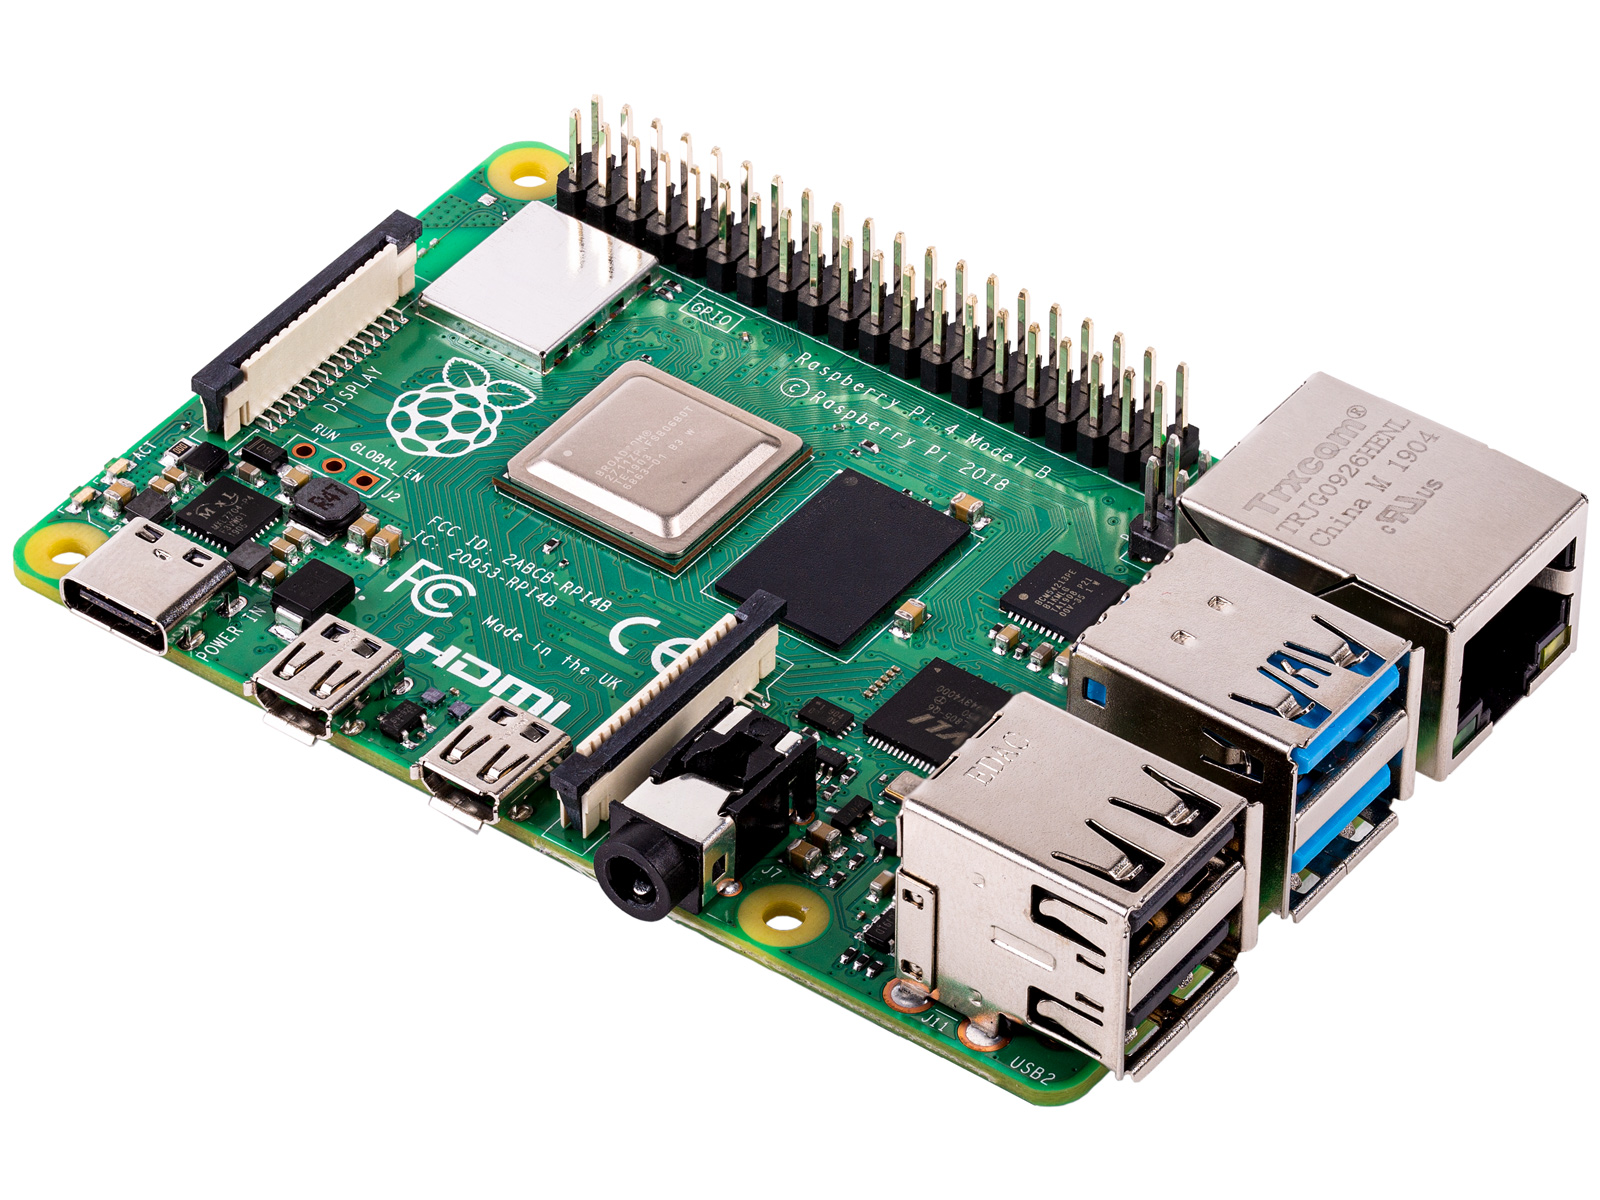
\includegraphics[width=\textwidth]{pi-4.jpg}}
				\caption*{Raspberry Pi Model 4}
			\end{subfigure}
		\hspace{\fill}
		\begin{subfigure}[b]{0.3\textwidth}
				\frame{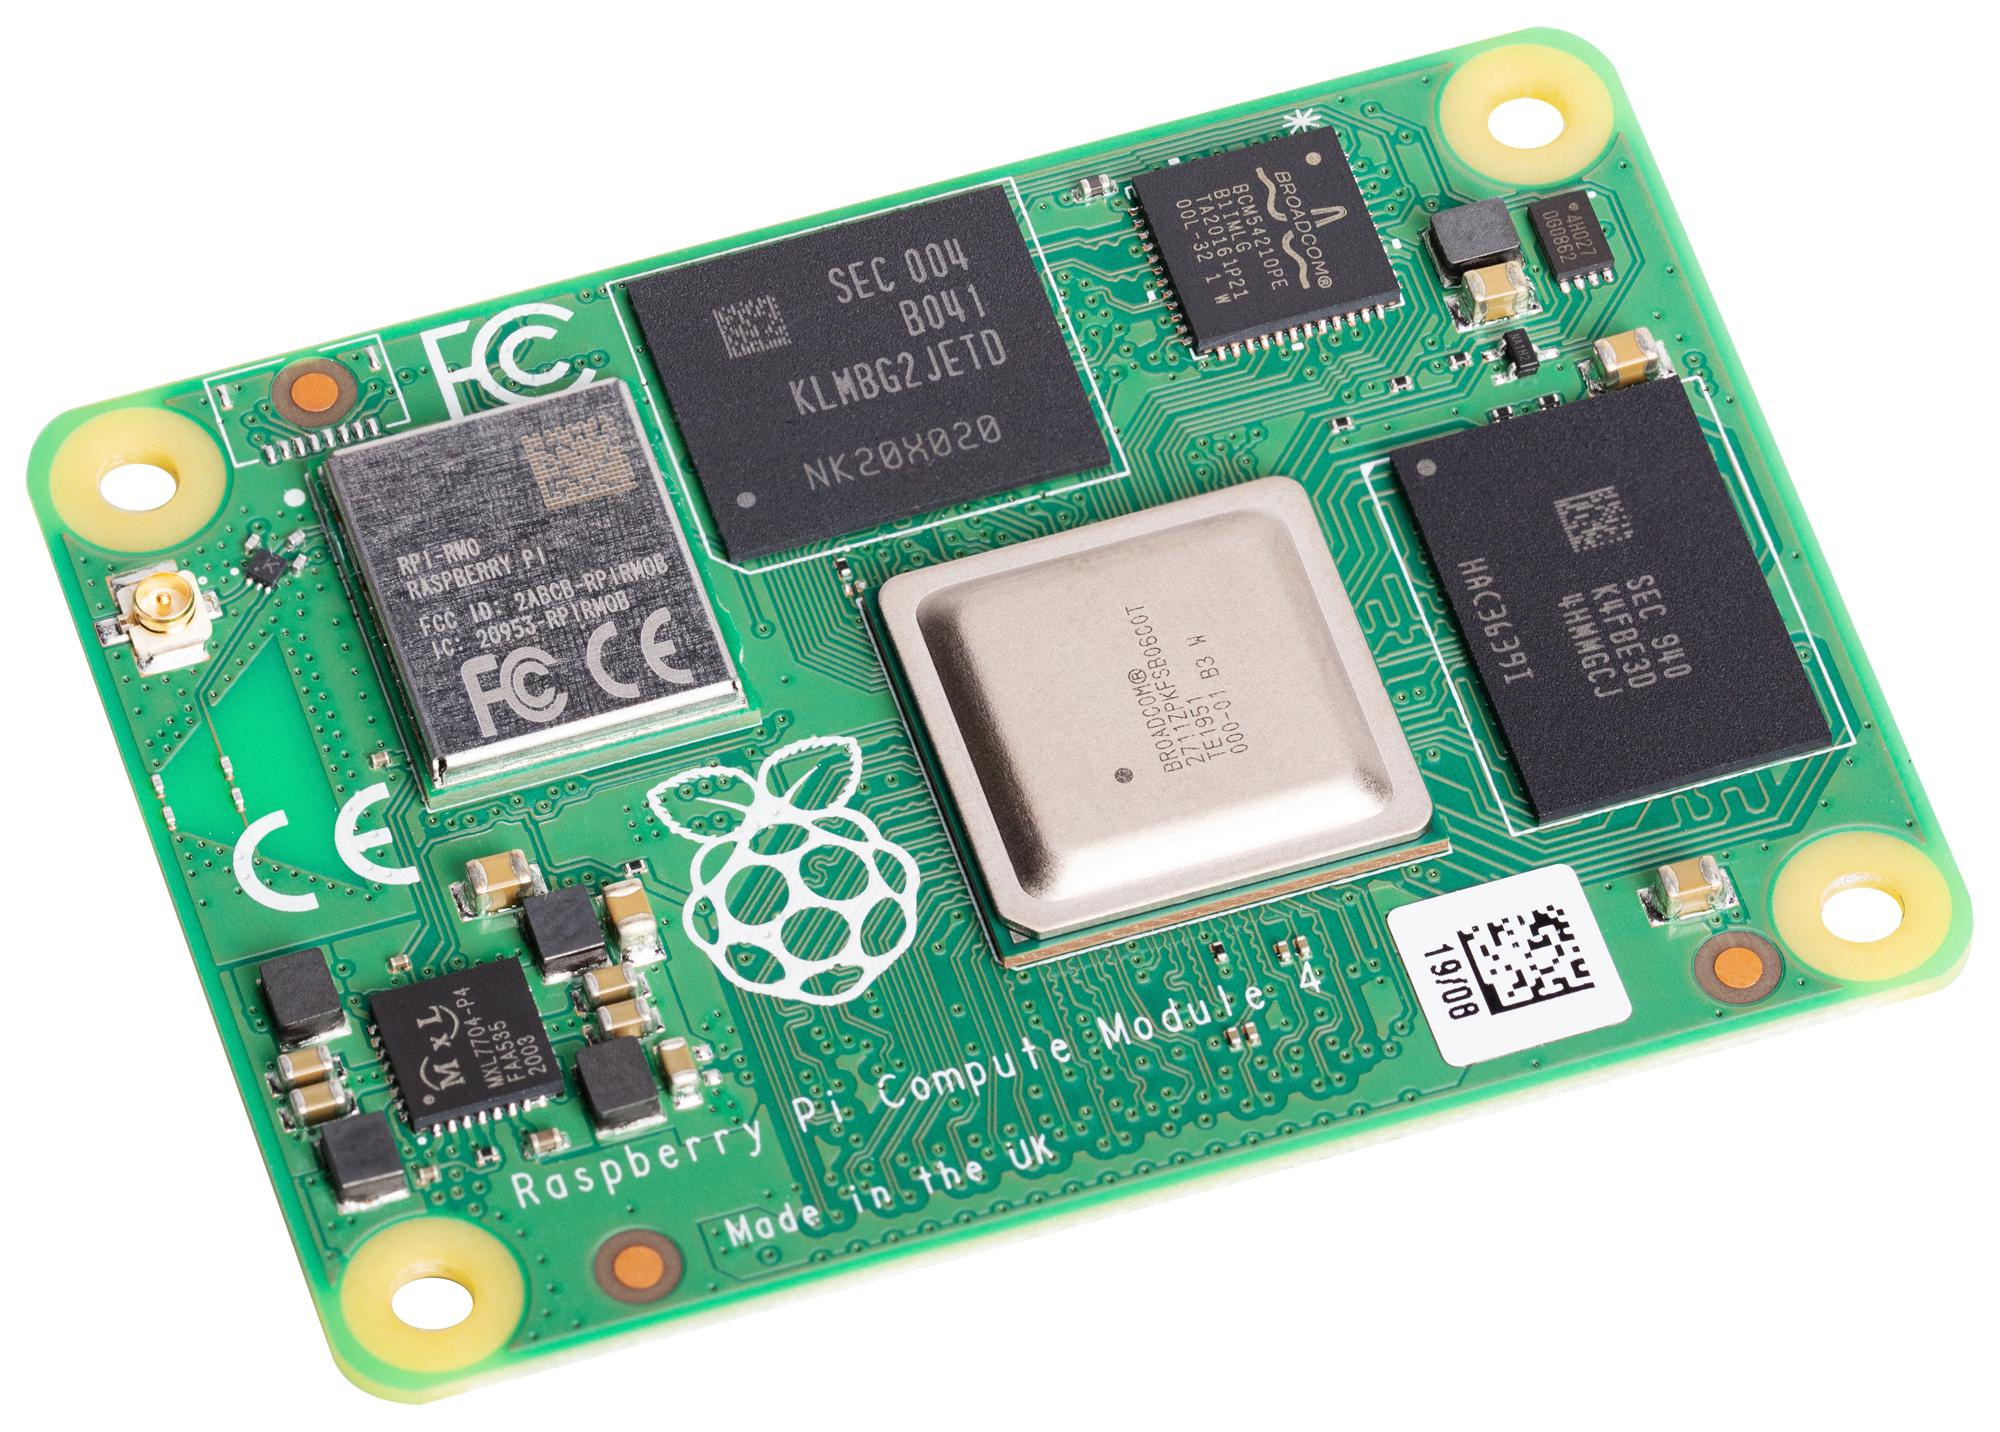
\includegraphics[width=\textwidth]{pi-cm.jpg}}
				\caption*{Raspberry Pi Compute Module 4}
			\end{subfigure}
		\hspace{\fill}
		\begin{subfigure}[b]{0.35\textwidth}
				\frame{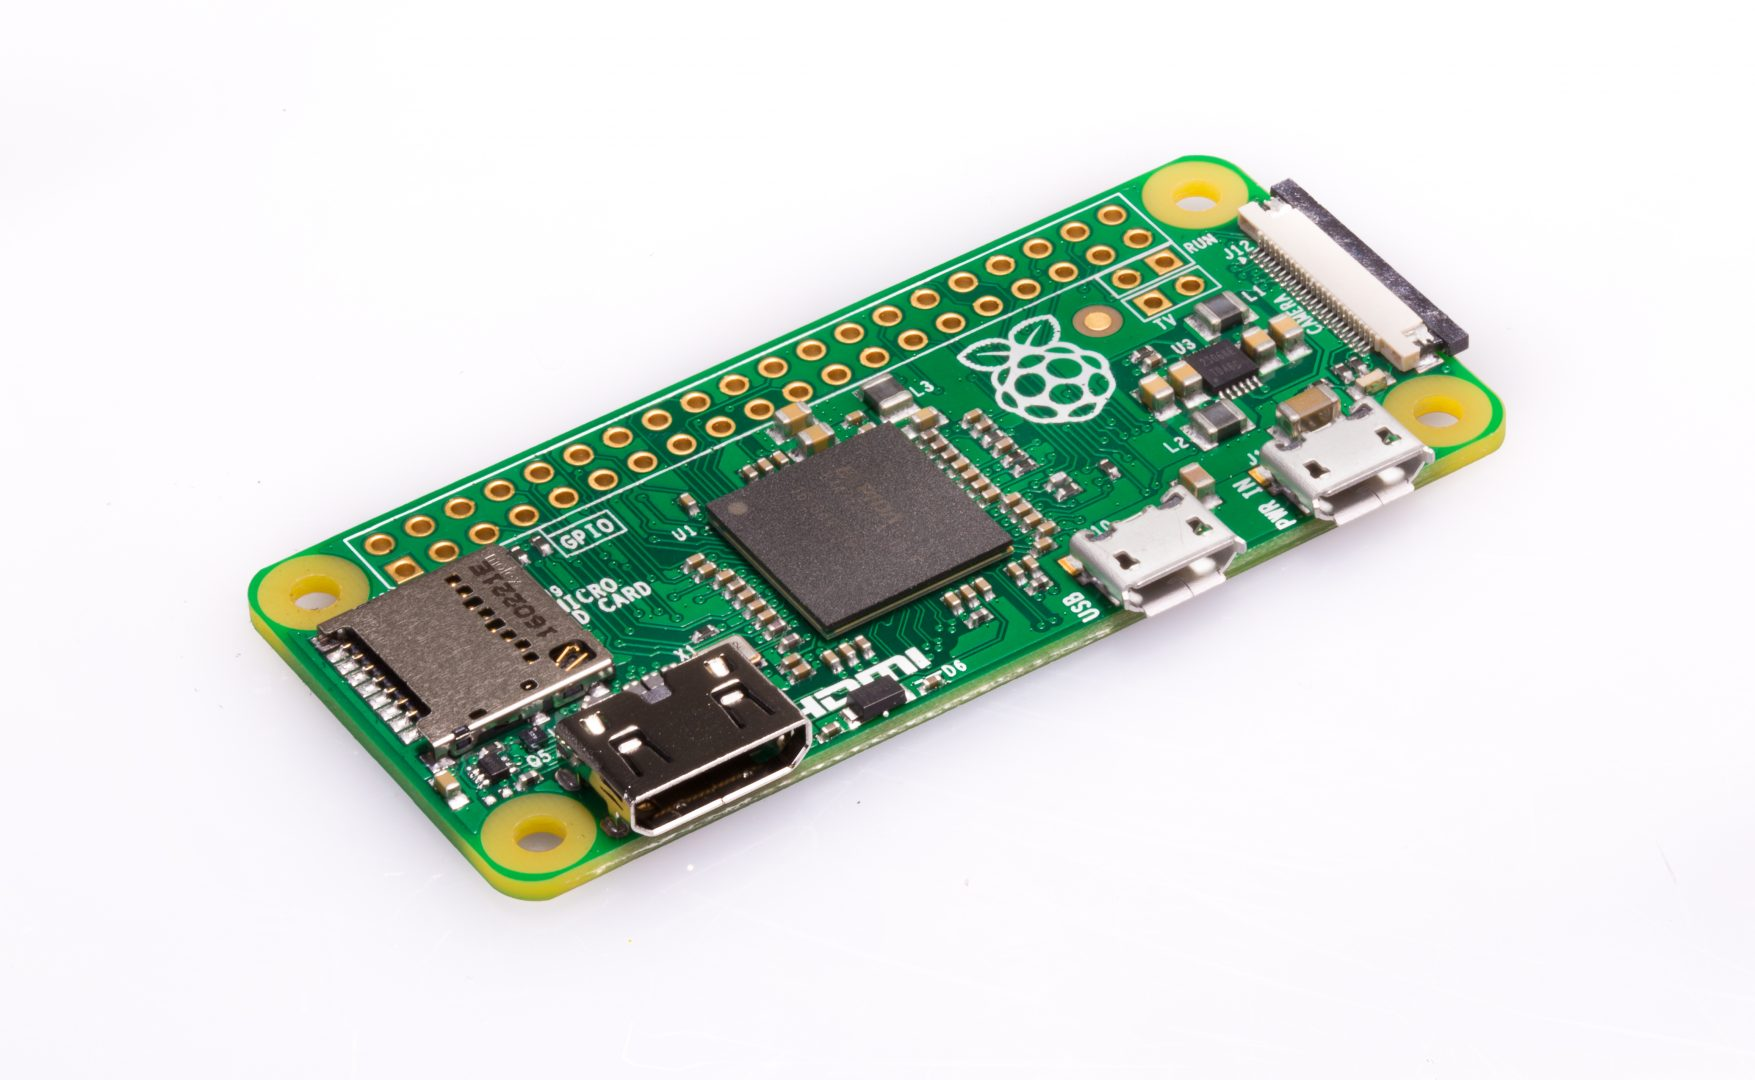
\includegraphics[width=\textwidth]{pi-zero.jpg}}
				\caption*{Raspberry Pi Zero Wireless}
			\end{subfigure}
	\end{figure}
\end{frame}

\begin{frame}{\insertsectionhead}
	\framesubtitle{Ciri Khas Utama \textit{Single Board Computer}}
	\justifying
	\textit{Single Board Computer} memiliki satu ciri utama di mana tempat pemrosesannya dilakukan di satu chip yang disebut dengan \textbf{mikroprosesor}. Meskipun berukuran kecil, satu mikroprosesor dapat memiliki kecepatan pemrosesan hingga 1,5 GHz.
	\vfill
	\begin{block}{Info}
		\textit{\textbf{Broadcom}} merupakan supplier utama mikroprosesor perangkat \textit{\textbf{Raspberry Pi}} dengan model \textit{\textbf{BCM2835}} hingga \textit{\textbf{BCM2711}}
	\end{block}
\end{frame}

\begin{frame}{\insertsectionhead}
	\framesubtitle{Arsitektur Lain \textit{Internet of Things}}
	\justifying
	Selain menggunakan mikroprosesor, beberapa perangkat IoT juga menggunakan teknologi \textbf{mikrokontroler}. Dibandingkan dengan mikroprosesor, mikrokontroler dibuat untuk perang-kat IoT yang berukuran lebih \textit{compact} dan memiliki harga jauh lebih murah daripada mikroprosesor.
	\vfill
	Namun dalam hal pemrosesan, mikroprosesor tetap paling unggul dibandingkan mikrokontroler. Secara spesifikasi, mikrokontroler hanya bekerja dengan kecepatan \textit{clock} 133MHz.
	\vfill
	Jadi, Mikrokontroler atau Mikroprosesor?
\end{frame}

\begin{frame}{\insertsectionhead}
	\framesubtitle{Arsitektur Konektivitas \textit{Internet of Things}}
	\justifying
	Layaknya gawai cerdas, perangkat IoT juga dilengkapi dengan konektivitas perangkat baik nirkabel maupun kabel. Terdapat banyak cara yang dapat dilakukan oleh perangkat IoT untuk terhubung ke Internet.
	\vfill
	\begin{multicols}{2}
		\begin{itemize}
			\item \textit{Wireless Fidelity (Wi-Fi)}
			\item \textit{Ethernet}
			\item \textit{Bluetooth}
			\item \textit{LoRa}
		\end{itemize}
	\end{multicols}
	\vfill
	\begin{block}{Info}
		Tidak semua perangkat mendukung ini, beberapa menggunakan konsep modular yang dapat dipasang secara terpisah
	\end{block}
\end{frame}

\begin{frame}{\insertsectionhead}
	\framesubtitle{Nirkabel atau Kabel?}
	\justifying
	Sebagian besar perangkat IoT dibuat untuk lepas dari kekangan kabel LAN, sehingga dalam implementasinya banyak yang menggunakan teknologi nirkabel seperti Wi-Fi untuk jarak dekat dan LoRa untuk jarak sangat jauh.
	\vfill
	\begin{block}{Info}
		Teknologi \textit{LoRa} dapat menjangkau hingga radius 10 mil atau kurang lebih 15km dari titik asal. Sehingga sangat cocok digunakan di area pegunungan
	\end{block}
\end{frame}

\begin{frame}{\insertsectionhead}
	\framesubtitle{Jangkauan \textit{LoRa}}
	\justifying
	\begin{figure}[ht!]
		\begin{subfigure}[b]{0.6\textwidth}
			\frame{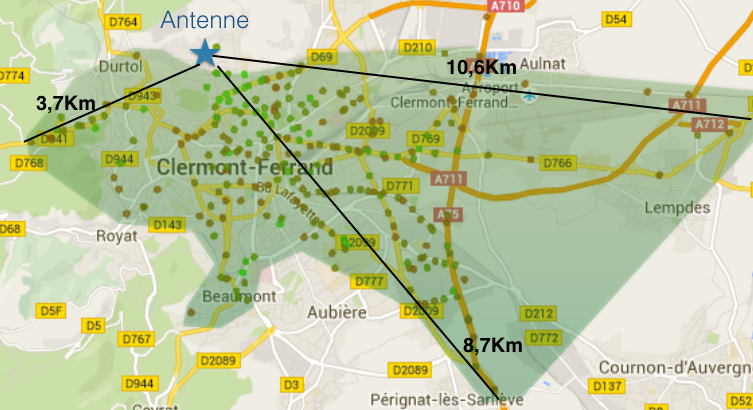
\includegraphics[width=\textwidth]{peta-jangkauan.png}}
			\caption*{Dalam eksperimen asli, \textit{LoRa} dapat menjangkau hingga 10km}
		\end{subfigure}
	\end{figure}
\end{frame}

\begin{frame}{\insertsectionhead}
	\framesubtitle{IPv4 atau IPv6?}
	\justifying
	Layaknya komputer pada biasanya, semua perangkat IoT diwajibkan untuk memiliki alamat IP agar bisa terhubung ke Internet. Tanpa adanya alamat IP satu perangkat IoT tidak akan terhubung ke jaringan manapun.
	\vfill
	Pada dasarnya semua perangkat IoT sudah mendukung pengalamatan IPv4, namun tidak semua mendukung teknologi IPv6. Hanya perangkat-perangkat tertentu yang dapat menggunakan IPv6 seperti Raspberry Pi.
	\vfill
	\begin{block}{Info}
		Alamat IPv6 memiliki panjang mencapai 128-bit, sehingga memungkinkan setiap perangkat di seluruh dunia untuk memiliki alamat mereka masing-masing.
	\end{block}
\end{frame}

\begin{frame}{\insertsectionhead}
	\framesubtitle{TCP atau UDP?}
	\justifying
	Protokol merupakan aspek vital jika membicarakan mengenai komunikasi data. Karena keduanya memiliki perbedaan yang sangat mencolok, yang di mana TCP mengutamakan integritas data. Sedangkan UDP mengutamakan situasi real-time meski mengorbankan integritas data.
	\vfill
	Keduanya digunakan dalam kondisi-kondisi tertentu, seperti contoh:
	\begin{itemize}
		\item TCP digunakan untuk mengirimkan data penting dan vital
		\item UDP digunakan untuk mengirimkan data biasa namun memerlukan real-time
	\end{itemize}
\end{frame}

\begin{frame}{\insertsectionhead}
	\framesubtitle{TCP VS UDP}
	\justifying
	 \begin{figure}[ht!]
		\begin{subfigure}[b]{0.75\textwidth}
			\frame{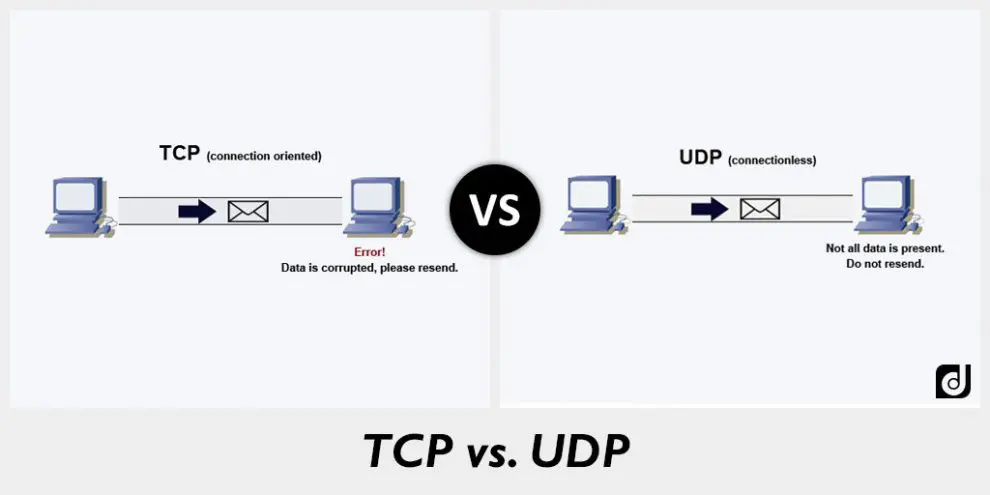
\includegraphics[width=\textwidth]{tcp-udp.png}}
		\end{subfigure}
	\end{figure}
\end{frame}

\begin{frame}{\insertsectionhead}
	\framesubtitle{Arsitektur Komunikasi \textit{Internet of Things}}
	\justifying
	Dalam hal berkomunikasi, perangkat \textit{Internet of Things} dapat menggunakan teknik komunikasi yang berbeda dari model biasanya. Di dunia Jaringan Komputer kita mengenal istilah \textbf{Client-Server} dan \textbf{Peer-to-Peer}. 
	\vfill
	Kedua teknik ini dapat digunakan dengan baik oleh teknologi IoT. Namun ada satu teknik baru yang mengandalkan pihak ketika atau \textit{Middleman}. Layaknya jual beli koran yang di mana \textbf{Penerbit} menjadi pengirim data, \textbf{Penjaja Koran} menjadi orang ketiga, dan \textbf{Pembeli} menjadi penerima data. Dikenal dengan istilah \textbf{\textit{Broker}}
\end{frame}

\begin{frame}{\insertsectionhead}
	\framesubtitle{Arsitektur Komunikasi \textit{Internet of Things}}
	\justifying
	  \begin{figure}[ht!]
		\begin{subfigure}[b]{0.3\textwidth}
				\frame{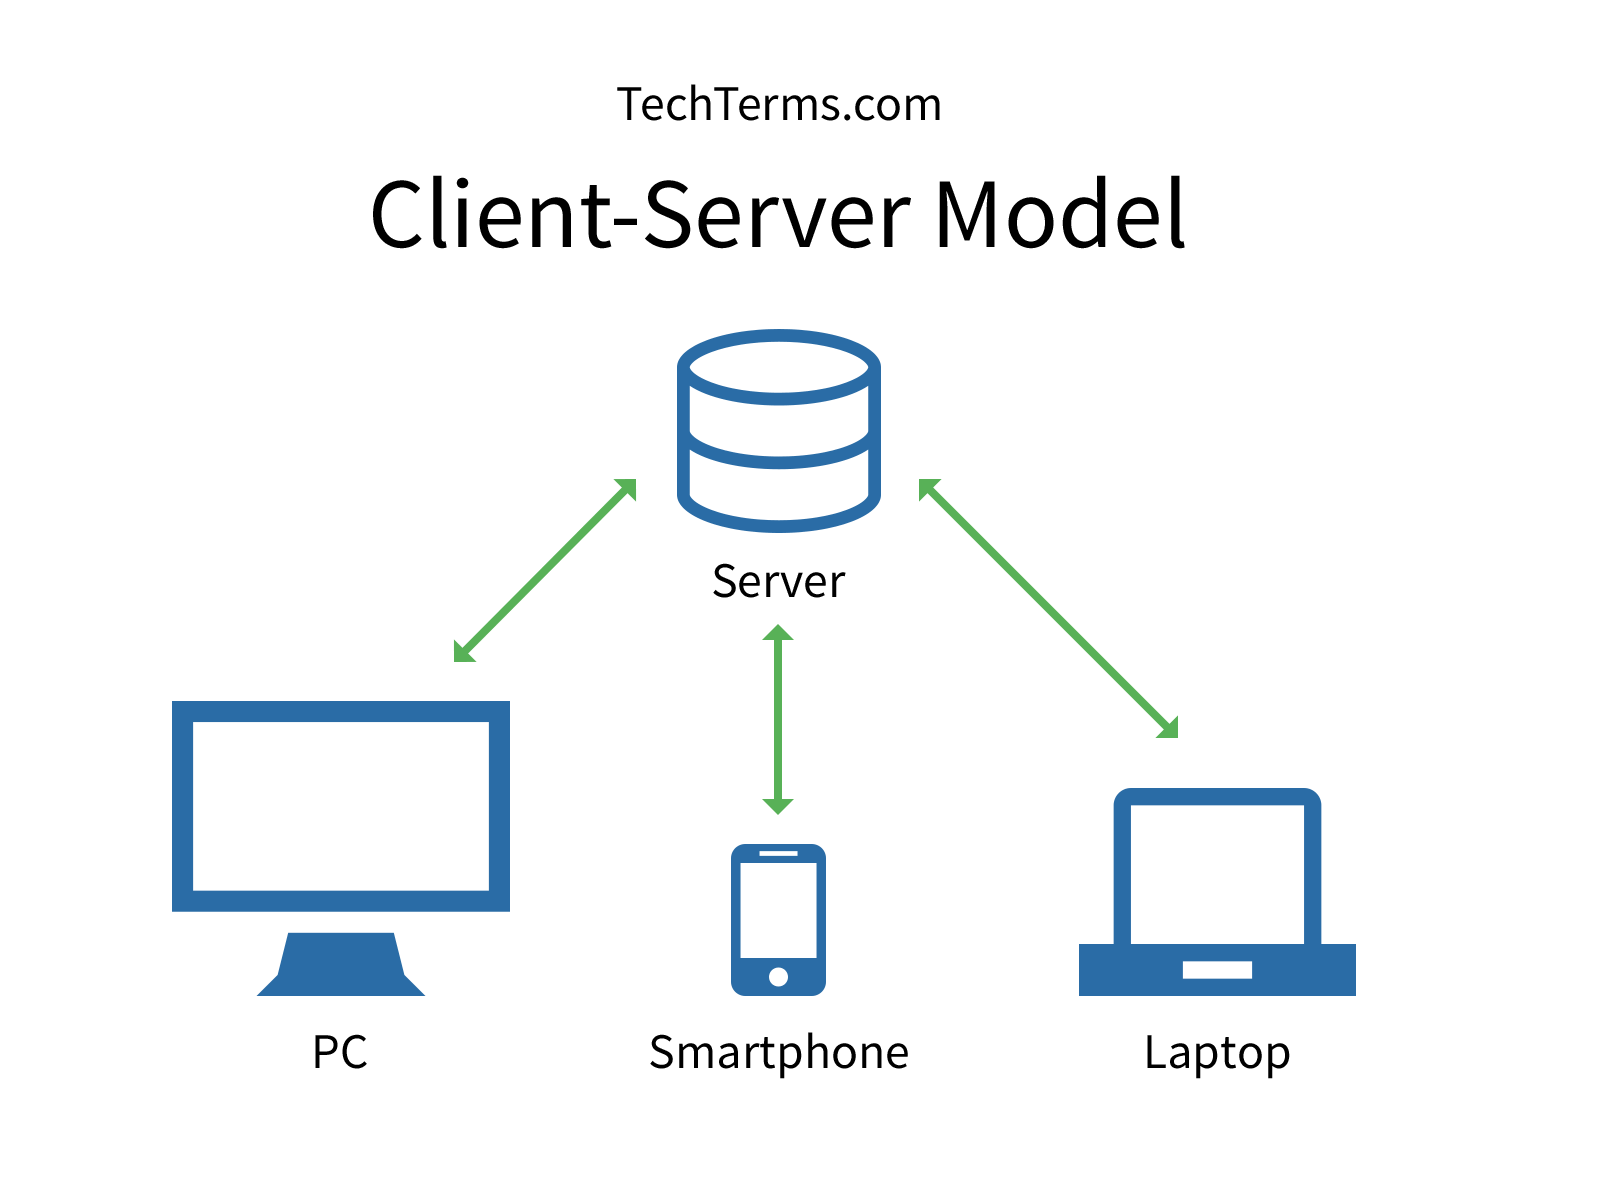
\includegraphics[width=\textwidth]{client-server.png}}
				\caption*{\textit{Client-Server}}
			\end{subfigure}
		\hspace{\fill}
		\begin{subfigure}[b]{0.3\textwidth}
				\frame{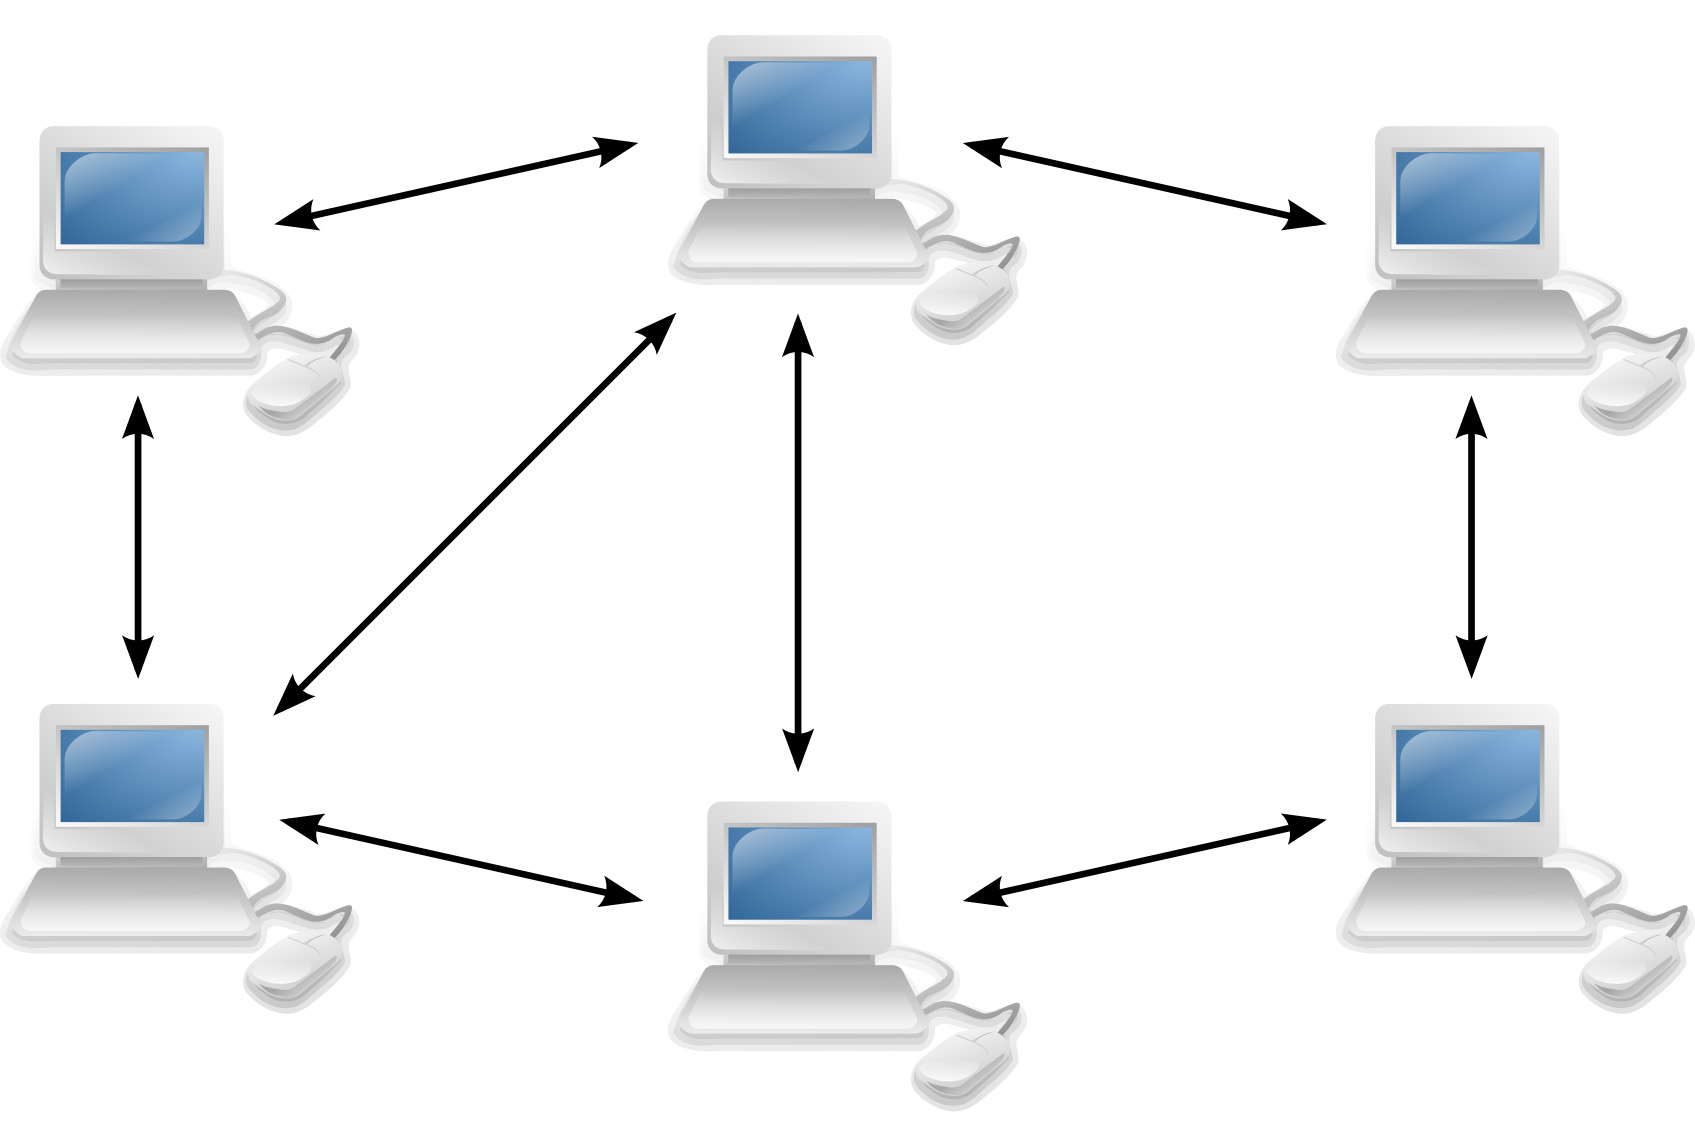
\includegraphics[width=\textwidth]{peer-to-peer.jpg}}
				\caption*{\textit{Peer-to-Peer}}
			\end{subfigure}
		\hspace{\fill}
		\begin{subfigure}[b]{0.35\textwidth}
				\frame{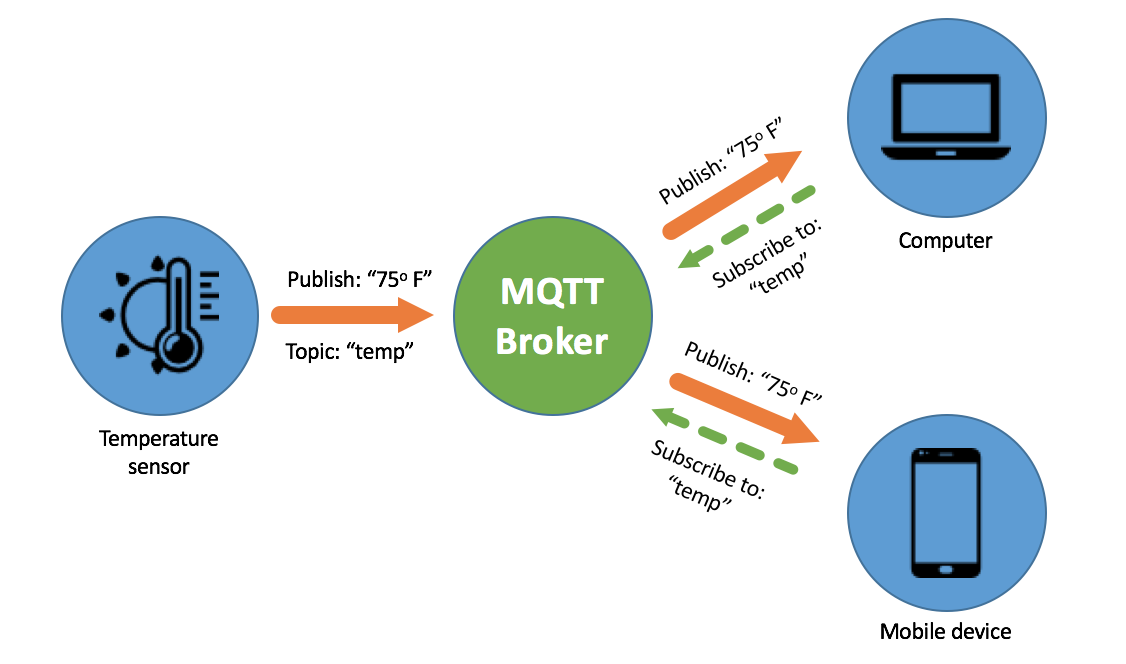
\includegraphics[width=\textwidth]{broker.png}}
				\caption*{\textit{Broker/Middleman}}
			\end{subfigure}
	\end{figure}
\end{frame}

\setbeamertemplate{background} 
{
	\includegraphics[width=\paperwidth,height=\paperheight]{thank-you.jpg}
}
\begin{frame}[plain]
\end{frame}